\documentclass[a4paper,16pt]{article}

%%% Работа с русским языком
\usepackage{cmap}					% поиск в PDF
\usepackage{mathtext} 				% русские буквы в фомулах
\usepackage[T2A]{fontenc}			% кодировка
\usepackage[utf8]{inputenc}			% кодировка исходного текста
\usepackage[english,russian]{babel}	% локализация и переносы

%%% Дополнительная работа с математикой
\usepackage{amsmath,amsfonts,amssymb,amsthm,mathtools} % AMS
\usepackage{icomma} % "Умная" запятая

%% Шрифты
\usepackage{euscript}	 % Шрифт Евклид
\usepackage{mathrsfs}    % Красивый матшрифт

%% Абзац
\usepackage{indentfirst}

%% Перенос знаков в формулах (по Львовскому)
\newcommand*{\hm}[1]{#1\nobreak\discretionary{}
{\hbox{$\mathsurround=0pt #1$}}{}}

%% Источники
\usepackage[nottoc]{tocbibind}

%% Вставка картинок
\usepackage{graphicx}
\graphicspath{{Picture/}}
\DeclareGraphicsExtensions{.pdf,.png,.jpg}

%% Работа с ссылками
\usepackage{url}
\usepackage{hyperref}

%% Работа с кодом
\usepackage{listings}
\usepackage{xcolor}

\definecolor{codegreen}{rgb}{0,0.6,0}
\definecolor{codegray}{rgb}{0.5,0.5,0.5}
\definecolor{codepurple}{rgb}{0.58,0,0.82}
\definecolor{backcolour}{rgb}{0.90,0.90,0.90}
\definecolor{keywordcolor}{RGB}{0,94,255}

\lstdefinestyle{mystyle}{
    backgroundcolor=\color{backcolour},   
    commentstyle=\color{codegreen},
    keywordstyle=\color{keywordcolor},
    numberstyle=\tiny\color{codegray},
    stringstyle=\color{codepurple},
    basicstyle=\ttfamily\footnotesize,
    breakatwhitespace=false,         
    breaklines=true,                 
    captionpos=b,                    
    keepspaces=true,                 
    numbers=left,                    
    numbersep=5pt,                  
    showspaces=false,                
    showstringspaces=false,
    showtabs=false,                  
    tabsize=2
}

\lstset{style=mystyle}

\title{lMovie}
\author{Александр Глушко, Денис Молдавский, \\ Михаил Сердюков, Валерий Айхенвальд}
\date{\today}

\begin{document}

\maketitle
\tableofcontents
\newpage

\section{Назначение}
\subsection{Функциональное назначение}
Проект представляет собой мобильное приложение для поиска фильмов и сериалов. Пользователь может создать аккаунт и добавлять туда понравившиеся фильмы, каждому добавленному фильму пользователь может присвоить статус и личный рейтинг. На базе выбранных фильмов и оценок программа рекомендует какие фильмы могут понравится пользователю. Предоставляется  возможность посмотреть основную информацию о каждом фильма, его награды, актеров и режиссера, рейтинг от пользователей приложения, а также найти кинотеатры в своем городе где данный фильм выходит в прокате и записаться на сеанс, купив билет.
\subsection{Эксплуатационное назначение}
Данное приложение будет интересно людям, которые часто ходят в кинотеатры, смотрят фильмы и сериалы дома. lMovie поможет вести свою личную картотеку фильмов, не потерять фильм о котором вы услышали и захотели посмотреть, а также не пропустить премьеру. Приложение ставит своей целью упростить поиск фильмов, кинотеатров и сеансов для пользователя. 


\section{Требования}
\subsection{Требования к вкладки список фильмов}
Приложение должно обеспечивать следующий функционал в данной вкладке:
\begin{enumerate}
    \item Просмотр фильмов отсортированных по некоторому набору правил:
    \begin{itemize}
        \item По названию
        \item По рейтингу
        \item По бюджету
        \item По дате выхода
    \end{itemize}
    \item Поиск фильмов по названию
    \item Просмотр списка фильмов отфильтрованных по:
    \begin{itemize}
        \item Жанру
        \item Году выпуска
        \item Актерам участвующим в фильме
        \item Режиссеру
        \item Студии издателю
        \item Полученным наградам
    \end{itemize}
    \item Просмотр основной информации по фильму:
    \begin{itemize}
        \item Название
        \item Год выпуска
        \item Режиссер
        \item Издатель
        \item Каст актеров
        \item Рейтинг
        \item Описание
        \item Кадры из фильма
        \item Награды фильма
    \end{itemize}
    \item Возможность одновременного использования сортировок и фильтров
    \item Возможность из карточки фильма перейти во вкладку с кинотеатрами с предустановленным фильтром на название выбранного фильма
    \item Реализовывать кнопку для добавления фильмов в личную коллекцию с разными статусами
\end{enumerate}
\subsection{Требования к вкладки список кинотеатров}
Приложение должно обеспечивать следующий функционал в данной вкладке:
\begin{enumerate}
    \item Возможность просмотра доступных кинотеатров в городе
    \item Просмотр кинотеатров отсортированных по некоторому правилу:
        \begin{itemize}
            \item Названию
            \item Среднему чеку
            \item Рейтингу
        \end{itemize}
    \item Поиск кинотеатров по названию
    \item Просмотр списка кинотеатров отфильтрованных по:
        \begin{itemize}
            \item Станции метро
            \item Фильму
        \end{itemize}
    \item Возможность по клику на кинотеатр перейти на выбор фильмов в этом кинотеатре, если не был установлен фильтр по фильмам. При установленном фильтре на фильмы по нажатию переход осуществляется в вкладку выбора времени для покупки.  
\end{enumerate}
\subsection{Требования к вкладки коллекция фильмов}
Приложение должно обеспечивать следующий функционал в данной вкладке:
\begin{enumerate}
    \item Возможность просмотра фильмов добавленных пользователем в личную коллекцию
    \item Просмотр фильмов отсортированных по некоторому набору правил:
    \begin{itemize}
        \item По названию
        \item По личному рейтингу
        \item По дате выхода
    \end{itemize}
    \item Поиск фильмов по названию
    \item Просмотр списка фильмов отфильтрованных по:
    \begin{itemize}
        \item Статусу присвоенному пользователем
        \item Жанру
        \item Году выпуска
        \item Актерам участвующим в фильме
        \item Режиссеру
        \item Студии издателю
        \item Полученным наградам
    \end{itemize}
    \item Возможность удалить фильм из коллекции
    \item Возможность добавить статус фильму из списка стандартных и списка статусов созданных пользователем
    \item Возможность создать собственный статус
\end{enumerate}
\subsection{Требования к вкладки профиль}
Приложение должно обеспечивать следующий функционал в данной вкладке:
\begin{enumerate}
    \item Просмотр данных о пользователе
    \item Возможность редактировать данные о пользователе
    \item Возможность выйти из аккаунта
    \item Возможность войти в систему под своими учетными данными
    \item Возможность зарегистрироваться, если у пользователся еще нет аккаунта
\end{enumerate}

\section{Проектирование модели данных}
\subsection{ER диаграмма}
На основе функциональных требований был выделен следующий набор сущностей и связей, который мы отобразили в виде ER диаграммы (рис. \ref{fig:ER}). Стоит заметить, что для избавления от слабых сущностей были добавлены id, уникальные идентификаторы объектов.
\begin{figure}[h]
    \centering
    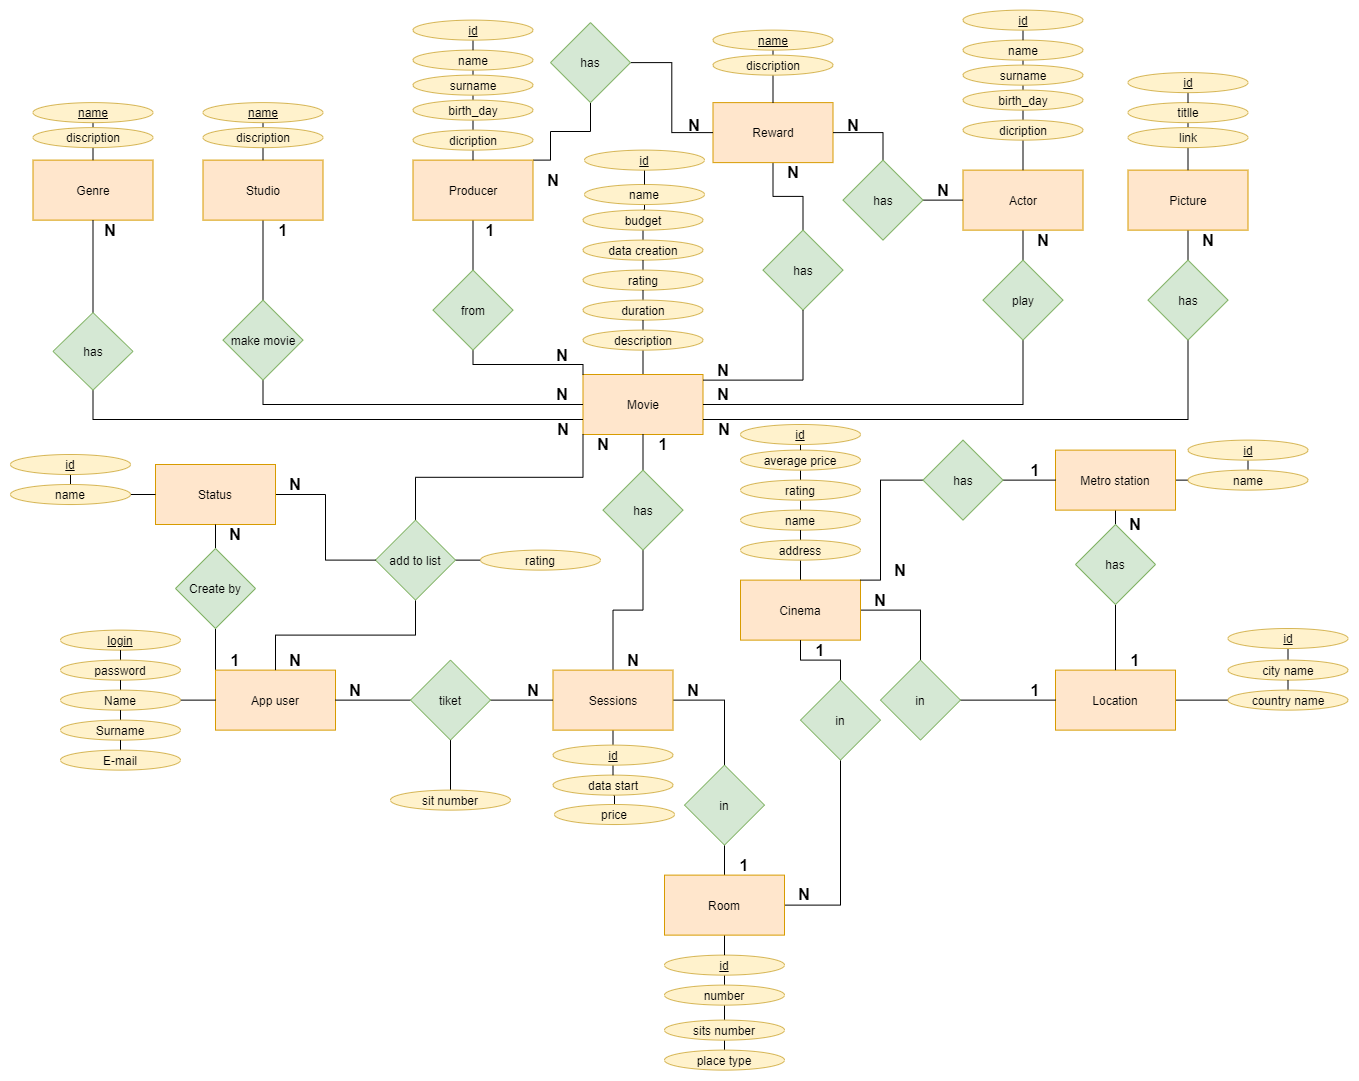
\includegraphics[scale=0.28]{thisMoview.png}
    \caption{ER Diagram}
    \label{fig:ER}
\end{figure}
\subsection{Текстовое описание ограничения наложенные на данные}
У каждого фильма обязательно, есть название, продюсер, дата создания и студия создавшая фильм, а также может присутствовать описание. К фильму обязательно относится один или несколько жанров и каст актеров. Для продюсера и актера обязательными полями являются имя, фамилия и день рождения, а также может присутствовать описание (краткая биография). Для жанра и студии обязательными полями является только имя, но может присутствовать и описание. Фильм, продюсер и актеры могут иметь одну или несколько наград, у награды обязательно есть название и описание.

Следующая ключевая сущность это пользователь. У пользователя обязательно есть логин, пароль, имя, фамилия и адрес электронной почты. Пользователь может добавлять один или несколько фильмов в свою коллекцию и по желанию выставлять им рейтинг, а так же присваивать один из предусмотренных статусов или создать свой новый статус. Пользователь может купить билет на сеанс, который обязательно содержит место. Сеанс содержит информацию о дате начала, цене и зале в котором он будет проходить. Зал в свою очередь содержит информацию о его номере, количестве мест и виде рассадки. Вид рассадки описывается в виде json объекта. Так же зал обязательно содержит информацию о кинотеатре в котором он проходит. Кинотеатр обязательно содержит информацию о своем названии, адресе и локации. Так же при наличии данной информации, кинотеатр может хранить в себе станцию метро, рейтинг и средний чек. Локация представляется в виде двух полей город и страна. Станция метро же имеет только название и ссылку на локацию в которой расположена.
\subsection{Нормализация}
При построении базы основной задачей ставилось получение 3 нормальной форму. Выбор на данную нормальную форму пал после прочтения книги Rex Hogan \cite{Norm} в которой он советует всегда при проектировки начинать с 3 нормальной форму, как с гипотетического решения и далее только при необходимости переходить на 4 и 5, которые используется реже в промышленных решениях. При нормализации мы так же хотели избавится от аномалии с разными написанием названий городов, наград и тому подобного, поэтому старались по макаемому вынести все в справочники. Итоговая модель представлена на (рис. \ref{fig:tables}).

\begin{figure}[h]
    \centering
    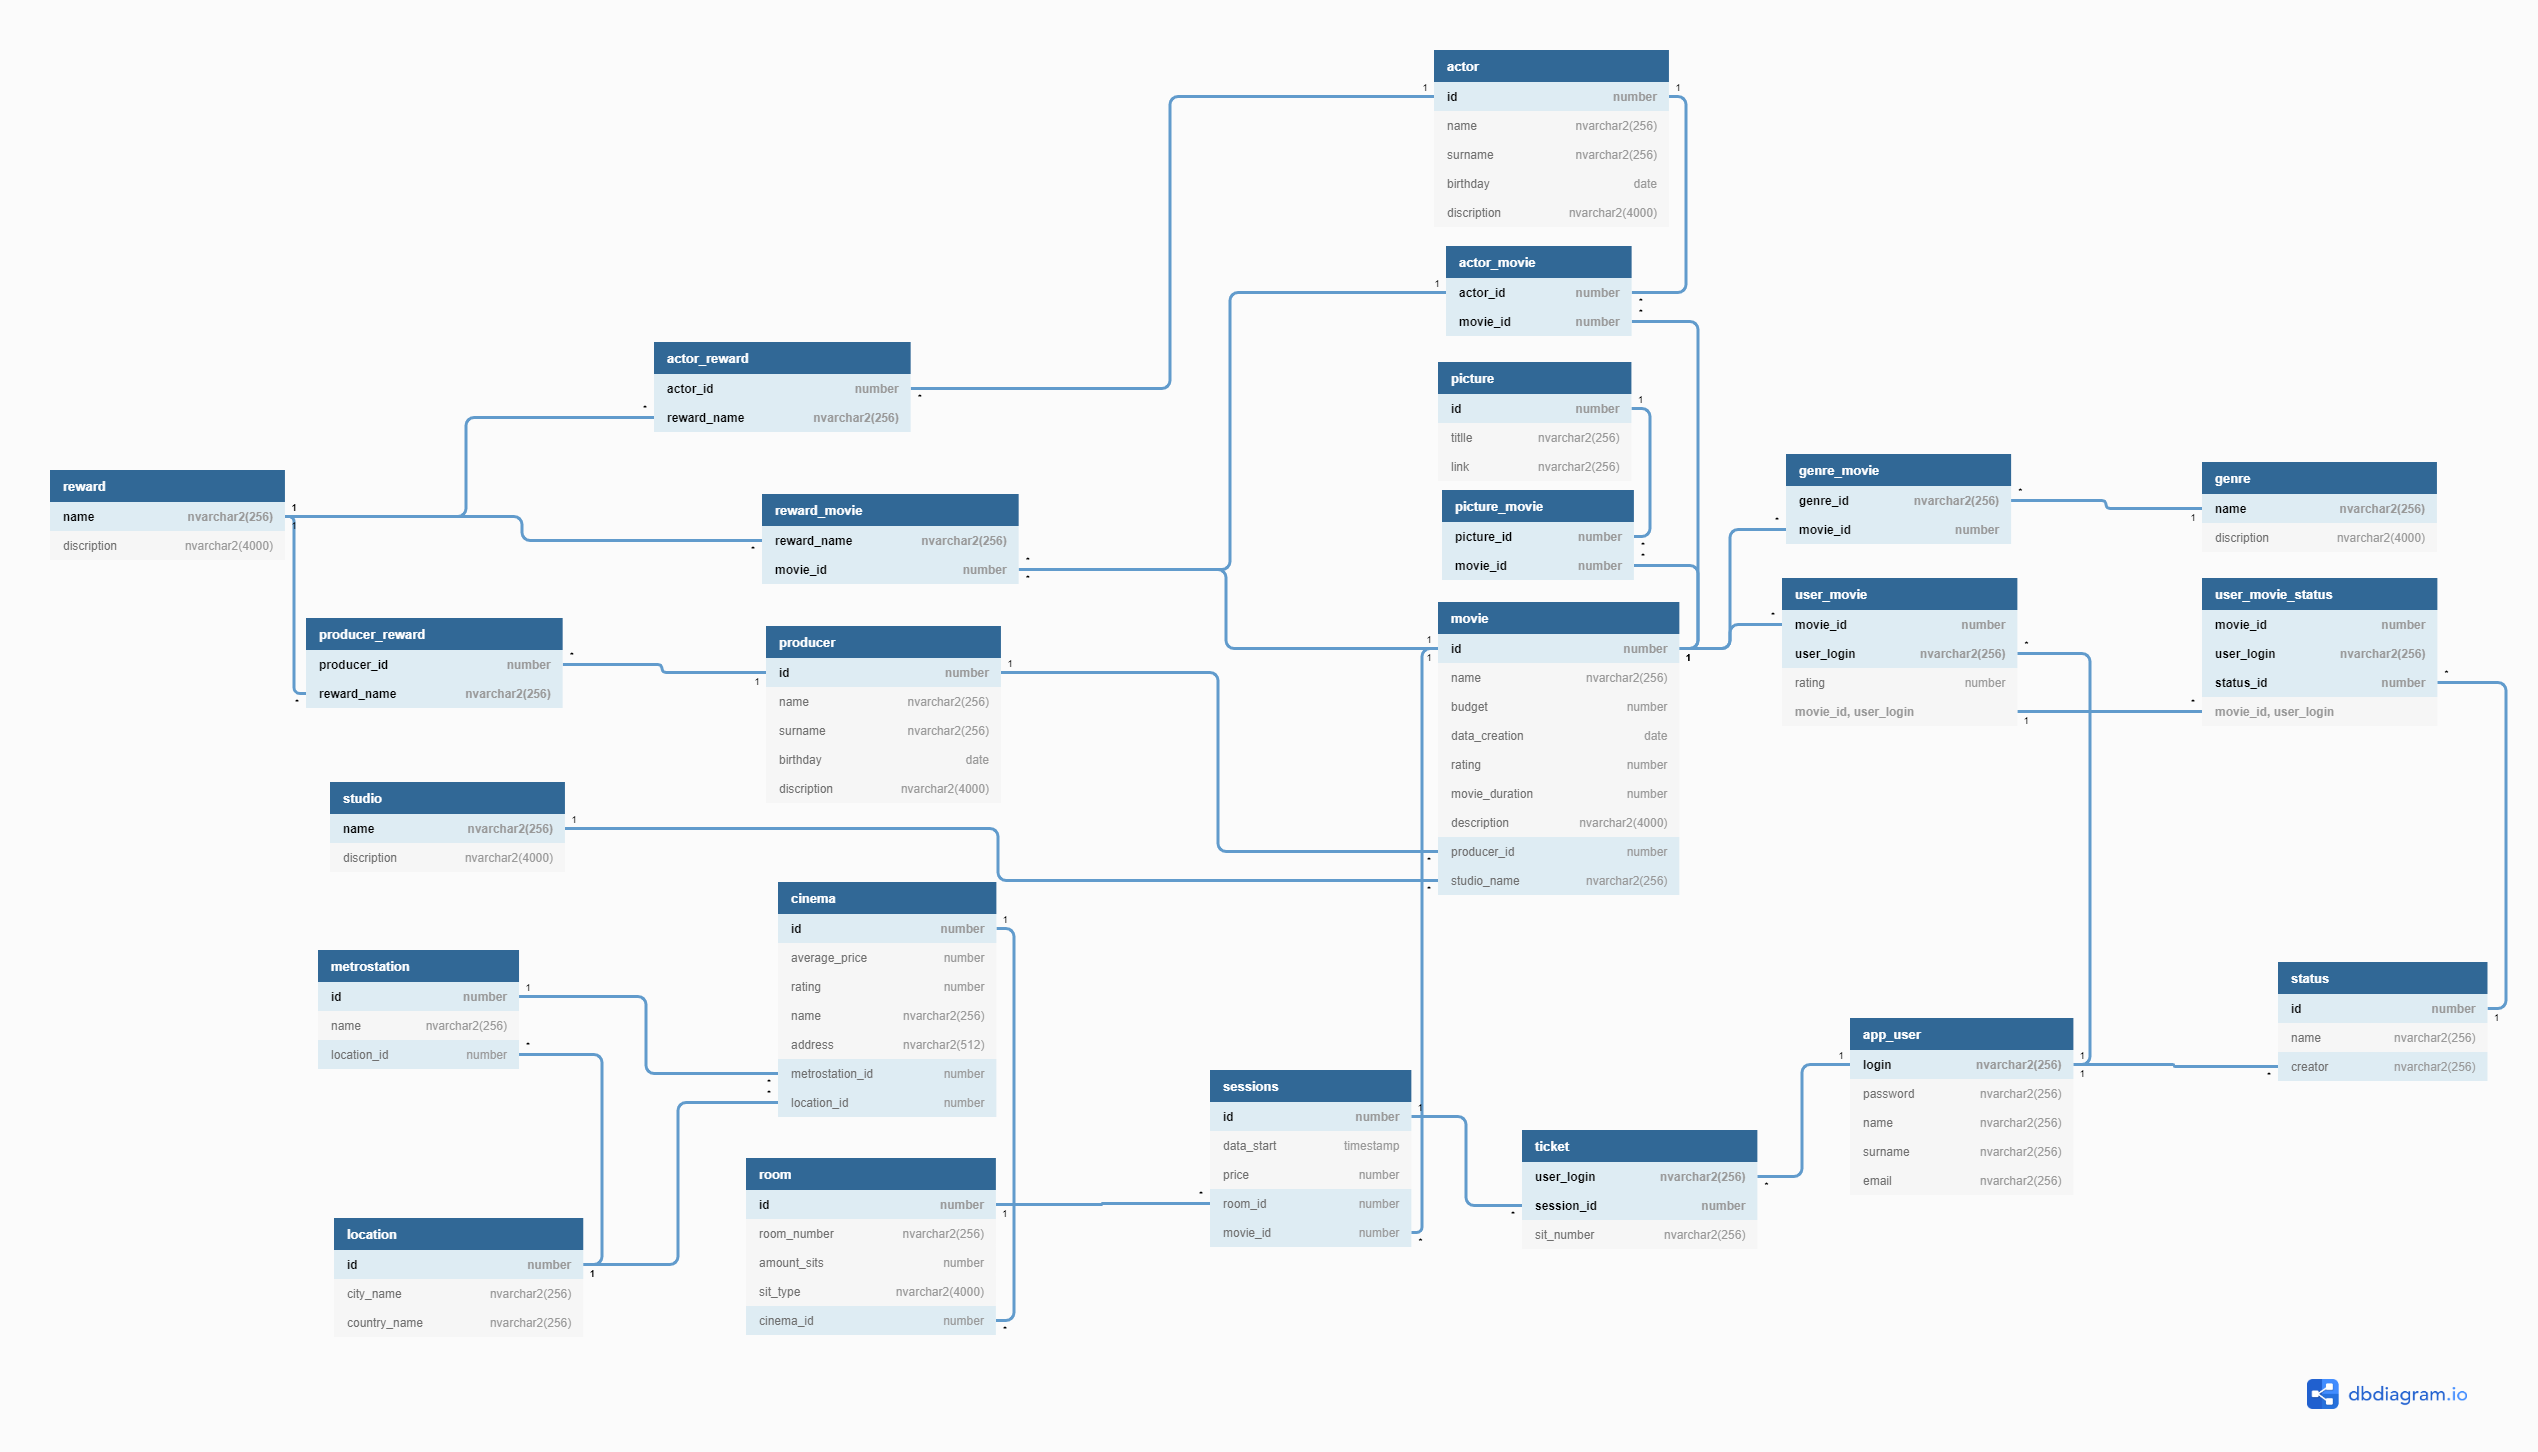
\includegraphics[scale=0.15]{iMovie db.png}
    \caption{Table Diagram}
    \label{fig:tables}
\end{figure}

\subsection{SQL DDL script}
\begin{lstlisting}[language=SQL]
-- drop table reward_movie;
-- drop table picture_movie;
-- drop table actor_movie;
-- drop table actor_reward;
-- drop table producer_reward;
-- drop table genre_movie;
-- drop table user_movie_status;
-- drop table user_movie;
-- drop table ticket;
-- drop table sessions;
-- drop table room;
-- drop table movie;
-- drop table cinema;
-- drop table picture;
-- drop table reward;
-- drop table actor;
-- drop table producer;
-- drop table studio;
-- drop table genre;
-- drop table status;
-- drop table app_user;
-- drop table metrostation;
-- drop table location;

create table location (
    id number primary key not null,
    city_name nvarchar2(256) not null,
    country_name nvarchar2(256) not null
);

create table metrostation (
    id number primary key not null,
    name nvarchar2(256) not null,
    location_id number not null,
    foreign key (location_id) references location (id)
);

create table app_user (
    login nvarchar2(256) primary key not null,
    password nvarchar2(256) not null,
    name nvarchar2(256) not null,
    surname nvarchar2(256) not null,
    email nvarchar2(256) not null
);

create table status (
    id number primary key not null,
    name nvarchar2(256) not null,
    creator nvarchar2(256) not null,
    foreign key (creator) references app_user (login)
);

create table genre (
    name nvarchar2(256) primary key not null,
    discription nvarchar2(4000)
);

create table studio (
    name nvarchar2(256) primary key not null,
    discription nvarchar2(4000)
);

create table producer (
    id number primary key not null,
    name nvarchar2(256) not null,
    surname nvarchar2(256) not null,
    birthday date not null,
    discription nvarchar2(4000)
);

create table actor (
    id number primary key not null,
    name nvarchar2(256) not null,
    surname nvarchar2(256) not null,
    birthday date not null,
    discription nvarchar2(4000)
);

create table reward (
    name nvarchar2(256) primary key not null,
    discription nvarchar2(4000) not null
);

create table picture (
    id number primary key not null,
    titlle nvarchar2(256) not null,
    link nvarchar2(256)
);

create table cinema (
    id number primary key not null,
    average_price number,
    rating number,
    name nvarchar2(256) not null,
    address nvarchar2(512) not null,
    metrostation_id number,
    location_id number not null, 
    foreign key (metrostation_id) references metrostation (id),
    foreign key (location_id) references location (id)
);

create table room (
    id number primary key not null,
    room_number nvarchar2(256) not null,
    amount_sits number not null,
    sit_type nvarchar2(4000) not null, --Todo add json check
    cinema_id number not null,
    foreign key (cinema_id) references cinema (id)
);

create table movie (
    id number primary key not null,
    name nvarchar2(256) not null,
    budget number,
    data_creation date not null,
    rating number,
    movie_duration number,
    description nvarchar2(4000),
    producer_id number not null,
    studio_name nvarchar2(256) not null,
    foreign key (producer_id) references producer (id),
    foreign key (studio_name) references studio (name)
);

create table sessions (
    id number primary key not null,
    data_start timestamp with local time zone not null,
    price number not null,
    room_id number not null,
    movie_id number not null,
    foreign key (movie_id) references movie (id),
    foreign key (room_id) references room (id)
);

create table ticket (
    user_login nvarchar2(256) not null,
    session_id number not null,
    sit_number nvarchar2(256) not null,
    constraint user_session_pk primary key (user_login, session_id),
    foreign key (user_login) references app_user (login),
    foreign key (session_id) references sessions (id)
);

create table user_movie (
    movie_id number not null,
    user_login nvarchar2(256) not null,
    rating number,
    constraint user_movie_pk primary key (movie_id, user_login),
    foreign key (user_login) references app_user (login),
    foreign key (movie_id) references movie (id)
);

create table user_movie_status (
    movie_id number not null,
    user_login nvarchar2(256) not null,
    status_id number,
    constraint user_movie_status_pk primary key (movie_id, user_login, status_id),
    foreign key (movie_id, user_login) references user_movie (movie_id, user_login),
    foreign key (status_id) references status (id)
);

create table genre_movie (
    genre_id nvarchar2(256) not null,
    movie_id number not null,
    constraint genre_movie_pk primary key (genre_id, movie_id),
    foreign key (genre_id) references genre (name),
    foreign key (movie_id) references movie (id)
);

create table producer_reward (
    producer_id number not null,
    reward_name nvarchar2(256) not null, 
    constraint producer_reward_pk primary key (producer_id, reward_name),
    foreign key (producer_id) references producer (id),
    foreign key (reward_name) references reward (name)
);

create table actor_reward (
    actor_id number not null,
    reward_name nvarchar2(256) not null,
    constraint actor_reward_pk primary key (actor_id, reward_name),
    foreign key (actor_id) references actor (id),
    foreign key (reward_name) references reward (name)
);

create table actor_movie (
    actor_id number not null,
    movie_id number not null,
    constraint actor_movie_pk primary key (actor_id, movie_id),
    foreign key (actor_id) references actor (id),
    foreign key (movie_id) references movie (id)
);

create table picture_movie (
    picture_id number not null,
    movie_id number not null,
    constraint picture_movie_pk primary key (picture_id, movie_id),
    foreign key (picture_id) references picture (id),
    foreign key (movie_id) references movie (id)
);

create table reward_movie (
    reward_name nvarchar2(256) not null,
    movie_id number not null,
    constraint reward_movie_pk primary key (reward_name, movie_id),
    foreign key (reward_name) references reward (name),
    foreign key (movie_id) references movie (id)
);
\end{lstlisting}

\section{Запросы}
\subsection{Запросы для вкладки список фильмов}
\subsection{Запросы для вкладки список кинотеатров}
\subsection{Запросы для вкладки коллекция фильмов}
\subsection{Запросы для вкладки профиль}

\bibliographystyle{unsrt}                                   
\bibliography{references}

\end{document}

